%#BIBTEX bibtex KI
\documentclass{PoS}
\bibliographystyle{unsrt}
\usepackage{aas_macros}
\usepackage{amsmath}
\usepackage{graphicx}
\usepackage{amsfonts}
\usepackage{amssymb}

\author{Kiyotomo Ichiki\\
Kobayashi-Maskawa Institute for the Origin of Particles and
the Universe, Nagoya University, Chikusa-ku, Nagoya, 464-8602, Japan\\
E-mail: \email{ichiki@a.phys.nagoya-u.ac.jp}}

\title{21 cm signal from the PMFs (a draft prepared as a part of sec.~3
``constraining new physics from heating'')}

\abstract{\bf I am more than happy if you could include the sentences below
in section 3. 
Please trim and polish up the draft. Thank you very much!}

\FullConference{
Advancing Astrophysics with the Square Kilometre Array\\
June 8-13, 2014\\
Giardini Naxos, Italy}
\ShortTitle{EoR/CD Cosmology}
\begin{document}


\maketitle 

\setcounter{section}{2}
\section{Constraining new physics from heating}

% \subsection{PMF definitions}
% Primordial magnetic fields (PMFs) has been intensively investigated in
% the literature as possible seeds for large scale magnetic fields
% observed in galaxies and clusters of galaxies (for a recent review, see
% \citep{2013A&ARv..21...62D}).  Magnetic fields in galaxies in high
% redshifts \citep{2008Natur.454..302B} and in void regions
% \citep{2010Sci...328...73N,2010ApJ...722L..39A,2013ApJ...771L..42T} can
% well be the pieces of evidence that the seed fields are of primordial
% origin.  The primordial magnetic fields may be created in the very
% early universe, e.g., at the epoch of inflation, cosmological phase
% transition, and cosmological recombination.  From the practical
% viewpoint, it is often assumed that the stochastic primordial magnetic
% fields have the power-law spectrum of the form:
% \begin{equation}
% \left<
%  B_i({\bf k})B^*_j({\bf k}^\prime) 
% \right>
% = 
% (2\pi)^3 \delta({\bf k}-{\bf
% k}^\prime)\frac{\delta_{ij}-\hat{k}_i\hat{k}_j}{2}Ak^{n_B}
% \label{Eq:KI1}
% \end{equation}
% where $n_B$ is the spectral index of the magnetic field spectrum. The
% amplitude $A$ is related to the magnetic field strength which is
% smoothed with a Gaussian filter over a comoving scale $\lambda$
% \begin{equation}
% B_\lambda^2 = \int^{\infty}_0 d\ln k e^{-k^2\lambda^2} \frac{k^3
%  P_B(k)}{2\pi^2}
% =\frac{A}{4\pi^2 \lambda^{n_B+3}k^{n_B}_{D}}\Gamma\left(\frac{n_B+3}{2}\right)
% \end{equation}
% where $k_D$ is the damping scale of the magnetic fields
% \cite{1998PhRvD..58h3502S,1998PhRvD..57.3264J}. The Planck collaboration
% recently places limits on the PMFs as $B_\lambda < 3.4$ nG and $n_B<0$
% from the temperature anisotropies on large and small angular scales \cite{2013arXiv1303.5076P}.

\subsection{21 cm signal from the PMFs}

Primordial magnetic fields (PMFs) has been intensively investigated in
the literature as possible seeds for large scale magnetic fields
observed in galaxies and clusters of galaxies (for a recent review, see
\cite{2013A&ARv..21...62D}).  Magnetic fields in galaxies in high
redshifts \cite{2008Natur.454..302B} and in void regions
\cite{2010Sci...328...73N,2010ApJ...722L..39A,2013ApJ...771L..42T} can
well be the pieces of evidence that the seed fields are of primordial
origin.  The primordial magnetic fields may be created in the very
early universe, e.g., at the epoch of inflation, cosmological phase
transition, and cosmological recombination.  
The Planck collaboration
recently places limits on the PMFs as $B_{\lambda=1{\rm Mpc}} < 3.4$ nG and $n_B<0$
from the temperature anisotropies on large and small angular scales
\cite{2013arXiv1303.5076P}. 

The CMB brightness temperature fluctuations produced by the neutral
hydrogen 21-cm line (21 cm) would offer a new probe of the primordial
magnetic fields (PMFs) created in the early universe. For the 21 cm
observation, aside from the early structure formation effect by the
Lorentz force from the PMFs, one of the important effects is the
dissipation process of the PMFs that increases the baryon
temperature. The dissipation occurs mainly through the ambipolar
diffusion due to the velocity difference between neutral hydrogen (which
is the dominant component in the dark ages) and ionized particles (whose
trajectory is bent by the Lorentz force).  The effect of the dissipation
is rather significant. The gas temperature can reach $1000$ K or even
$10^4$ K at $z=30$ if the magnetic fields have the strength of
$B_\lambda \sim 3$ nG
\cite{2005MNRAS.356..778S,2006MNRAS.372.1060T,2009ApJ...692..236S,2014JCAP...01..009K}.

This dissipation will give rise to a unique signature of the PMFs on the
21 cm observation. Because the spin temperature is closely coupled to
the gas temperature at high redshift ($z>30$), the 21 cm signal would
come as `emission' if the energy dissipation is efficient. In
Fig.~\ref{fig:KI1} the global HI signal with several magnetic field
strengths are shown. For cases with sufficient magnetic fields, say
$B\gtrsim 0.03$ nG, the signal is always emission against CMB while in
the standard $\Lambda$CDM model the signal would be absorption for the
frequency range of $f_\nu \lesssim 80$ MHz (corresponding to the signal
from redshift $z\gtrsim 20$).

We show the angular power spectrum of the 21 cm brightness temperature
including the PMFs in Fig.~\ref{fig:KI2}
\cite{2014arXiv1403.2608S}. Here we do not account for any (standard)
heating effects (i.e., UV, X, and L$\alpha$ background emissions) to isolate and
clarify the effects from the PMFs.  On large scales which may be
relevant to SKA 
observations, there are two distinct contributions. One is from the
standard (adiabatic) density fluctuations enhanced by the heating from
the PMFs, and the other is from the PMF induced density fluctuations
dominant on smaller scales
\cite{2006MNRAS.372.1060T,2009ApJ...692..236S}. We can see from the
figure that $B=1$ nG
magnetic fields are marginally within reach for a statistical detection
of the power spectrum. Stacking observing channels in principle will add
more statistical power.

The angular correlation function in real space including the effects
from the PMFs is also studied in \cite{2009JCAP...11..021S}.  The
function exhibits a distinct feature because the PMFs induce early
structure formation and the small scale halos form more compared to the
case in the standard $\Lambda$CDM model The signal from primordial
magnetic fields shows oscillatory feature contrary to that in the
standard $\Lambda$CDM since the matter power spectrum induced by the
PMFs is blue and most of halos are formed at the scale close to the
magnetic Jeans' length. It has been argued that $5$ sigma detection of
the $0.5$ nG magnetic fields will be possible with less than one week
integration of SKA observation \cite{2009JCAP...11..021S}.

\begin{figure}[]
\includegraphics[width=0.6\linewidth,angle=0]{figs/KI_fig1.eps}
\caption{The global 21 cm signal with magnetic field strength $B=1$
$0.1$, $0.03$, and $0.01$ nG (colored lines from top to bottom). The
solid line corresponds to the model without primordial magnetic fields.
Note that any other heating source than magnetic fields is neglected in
the figure.}  \label{fig:KI1}
\end{figure}

\begin{figure}[]
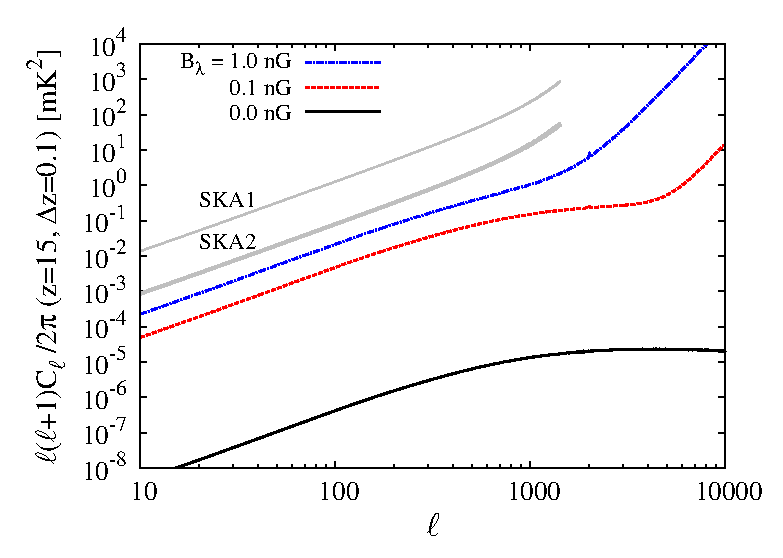
\includegraphics[width=0.6\linewidth,angle=0]{figs/KI_fig2.eps}
\caption{Angular power spectra for PMF strengths: $B=0,~ 0.1,~ 1.0$ nG
at $z=15$. The bottom curve shows the power spectrum from the standard
density perturbations for fully neutral medium without any heating and
reionization processes. The red and blue curves correspond to the cases
with heating by the PMFs with $B=0.1$ nG and $B=1.0$ nG,
respectively. The heating induces deviations of the spin temperature
from the CMB temperature and the signal is enhanced. The noise curves
for SKA1 and SKA2 are also shown as indicated. By courtesy of
M. Shiraishi \& H. Tashiro.}  \label{fig:KI2}
\end{figure}


\bibliography{KI.bib}
\end{document}
